\documentclass[10pt, a4paper, italian]{article}
\usepackage[T1]{fontenc}
\usepackage[utf8]{inputenc}
\usepackage{amsmath, amssymb, amsthm, thmtools, amsfonts, mathtools}
\usepackage{nicefrac}
\usepackage{calc}
\usepackage[pdftex, hyperindex, plainpages=false]{hyperref}
\usepackage[nameinlink]{cleveref} %load before classicthesis (clash)
%\usepackage[nochapters,pdfspacing]{classicthesis}
\usepackage{siunitx}
\usepackage[siunitx]{circuitikz}

\usepackage[a4paper]{geometry}
\usepackage{float}
\usepackage{mdframed}
\usepackage{titling}
\usepackage{booktabs}
\usepackage{graphicx}
\usepackage{caption, subcaption}
\usepackage{xcolor}
\usepackage[italian]{babel}
\usepackage{pgfplots}
\usepackage{listings}
%\usepackage{lmodern}
\usepackage{url}
\usepackage{enumitem}
\usepackage{tikz} %loads after classicthesis (xcolor incompat)

% lets graphicx know path where figures to be included are found
\graphicspath{{../figs/}}
\makeatletter
\def\input@path{{../figs/}}
%or: \def\input@path{{/path/to/folder/}{/path/to/other/folder/}}
\makeatother

% tikz pgf plots setup
\usepgfplotslibrary{external}
\pgfplotsset{compat=1.15}
%\tikzexternalize

% spaces and significant digits/figures for measurements
\sisetup{free-standing-units, space-before-unit, number-unit-product = \;,
scientific-notation = false, round-mode = figures, round-precision = 1,}

% turns all (hyperlinked) references black [default is blue]
\hypersetup{
	linktoc=all,
	colorlinks=true,
	linkcolor=black
}

% code listings config
%\lstset{
%language=Python,
%basicstyle=\ttfamily,
%columns=fullflexible,
%keepspaces=true,
%}

% mdframed (for boxed text) configuration
\mdfsetup{linewidth=0.6pt}

% Default fixed font does not support bold face
\DeclareFixedFont{\ttb}{T1}{txtt}{bx}{n}{12} % for bold
\DeclareFixedFont{\ttm}{T1}{txtt}{m}{n}{12}  % for normal

% Custom colors
\usepackage{color}
\definecolor{deepblue}{rgb}{0,0,0.5}
\definecolor{deepred}{rgb}{0.6,0,0}
\definecolor{deepgreen}{rgb}{0,0.5,0}

% Commands 
\newcommand{\executeiffilenewer}[3]{%
	\ifnum\pdfstrcmp{\pdffilemoddate{#1}}%
		{\pdffilemoddate{#2}}>0%
	{\immediate\write18{#3}}\fi%
}
% input .svg --> .pdf_tex graphs
%\newcommand{\includesvg}[1]{%
%	\executeiffilenewer{#1.svg}{#1.pdf}%
%	{inkscape -z -D --file=#1.svg %
%	--export-pdf=#1.pdf --export-latex}%
%	\input{#1.pdf_tex}%
%}
% Thanks UniPi's Department of Physics E. Fermi
\newcommand{\thanksdf}{(\thanks{Dipartimento di Fisica E.~Fermi,%
Universit\`a di Pisa - Pisa, Italy.}\;)}

% hyperlink to email address
\newcommand{\mail}[1]{\href{mailto:#1}{\textsf{#1}}}

% \vec for bold vectors, instead of overarrows (now "\arrvec")
\let\arrvec=\vec
\renewcommand{\vec}[1]{\boldsymbol #1}
% replaces straight phi with slanted phi
\renewcommand{\phi}{\varphi}
% replaces straight eps with curved epsilon
\newcommand{\eps}{\varepsilon}
% abbreviation for (sub_/super^)scripts of \lim, \sum,... in inline math
\newcommand{\ds}{\displaystyle}

% blackboard/number set letters
\newcommand{\CC}{\mathbb C}
\newcommand{\HH}{\mathbb H}
\newcommand{\KK}{\mathbb K}
\newcommand{\NN}{\mathbb N}
\newcommand{\PP}{\mathbb P}
\newcommand{\QQ}{\mathbb Q}
\newcommand{\RR}{\mathbb R}
\newcommand{\ZZ}{\mathbb Z}

\newcommand{\Abs}[1]{{\left\Vert #1\right\Vert}}
\newcommand{\enclose}[1]{{\left( #1 \right)}}
\newcommand{\Enclose}[1]{{\left[ #1 \right]}}
\newcommand{\floor}[1]{\left\lfloor #1 \right\rfloor}
\newcommand{\ceil}[1]{\left\lceil #1 \right\rceil}
\newcommand{\To}{\rightrightarrows}

% Math operators
\DeclareMathOperator{\divergence}{div}
\renewcommand{\div}{\divergence}
\DeclareMathOperator{\Imaginarypart}{Im}
\renewcommand{\Im}{\Imaginarypart}
\DeclareMathOperator{\Realpart}{Re}
\renewcommand{\Re}{\Realpart}
%\DeclareMathOperator{\arg}{arg}
\DeclareMathOperator{\tg}{tg}
\DeclareMathOperator{\arctg}{arctg}
\DeclareMathOperator{\settsinh}{settsinh}
\DeclareMathOperator{\settcosh}{settcosh}
\DeclareMathOperator{\tr}{tr}
\DeclareMathOperator{\im}{im}
\DeclareMathOperator{\sgn}{sgn}
\DeclareMathOperator{\diag}{diag}

\DeclarePairedDelimiter{\norm}{\lVert}{\rVert}
\DeclarePairedDelimiter{\scalar}{\langle}{\rangle}

% Logarithm with arbitrary base.
% -> log_10
\newcommand{\llog}[1][10]{\log_{#1}}

% Absolute value.
% -> |x|
\newcommand{\abs}[1]{\left| #1 \right|}

% Powers.
% -> x^a
\newcommand{\power}[2][2]{\left( #2 \right)^{#1}}

% Square.
% -> x^2
\newcommand{\sq}[1]{\power[2]{#1}}

% Expansion of the binomial coefficient.
% -> n1!/(n2!(n1 - n2)!)
\newcommand{\binomexpr}[2]{\frac{#1!}{#2!(#1 - #2)!}}

% Expression evaluation at a given point with square brackets.
% -> [x]_{a}
\newcommand{\at}[2]{\left[ #1\right]_{\makebox[-1pt][l]{${\scriptstyle#2}$}}}

% Expression evaluation in an interval.
% -> [x] _{a}^{b}
\newcommand{\eval}[3]{\left.#1%
  \right|_{\makebox[-1pt][l]{${\scriptstyle#2}$}}^{\makebox[-1pt][l]{${\scriptstyle#3}$}}}

% Upright d in math mode (for differentials).
% -> d
\newcommand{\ud}{\mathrm{d}}

% Differential.
% -> dx
\newcommand{\diff}[1][x]{\,\ud{#1}}

% Base command for defining derivatives.
% -> df/dx or d^kf/dx^k
\newcommand{\basederivative}[4][]{%
  \displaystyle%
  \ifx\\#1\\\frac{#4#2}{#4#3}%
  \else%
  \frac{#4^#1#2}{#4#3^#1}%
  \fi%
}

% Total derivative.
% -> df/dx(x) or d^kf/dx^k(x)
\newcommand{\td}[4][]{%
  \basederivative[#1]{#2}{#3}{\ud}%
  \ifx\\#4\\%
  \else%
  \mkern-4mu\left(#4\right)%
  \fi%
}

% Partial derivative.
% -> df/dx(x) or d^kf/dx^k(x)
\newcommand{\pd}[4][]{%
  \basederivative[#1]{#2}{#3}{\partial}%
  \ifx\\#4\\%
  \else%
  \mkern-4mu\left(#4\right)%
  \fi%
}

\newcommand{\intinf}{\int_{-\infty}^{\infty}\!\!\!}

\newcommand{\cinterval}[2]{\left[\, #1,~#2 \,\right]}

\newcommand{\linterval}[2]{\left[\, #1,~#2 \,\right)}

\newcommand{\rinterval}[2]{\left(\, #1,~#2 \,\right]}

\newcommand{\ointerval}[2]{\left(\, #1,~#2 \,\right)}

\newcommand{\prob}[1]{\displaystyle P\left(#1\right)}

\newcommand{\pvalue}{\emph{$p$-value}}

\newcommand{\cond}{\,|\,}

\newcommand{\expect}[1]{\displaystyle E\left[#1\right]}

\newcommand{\mom}[2][]{\displaystyle {\cal M}_{#2}\ifx\\#1\\\else(#1)\fi}

\newcommand{\momalg}[1]{\displaystyle \lambda_{#1}}

\newcommand{\momcen}[1]{\displaystyle \mu_{#1}}

\newcommand{\skewness}{\displaystyle \gamma_1}

\newcommand{\kurtosis}{\displaystyle \gamma_2}

\newcommand{\charf}[1][x]{\phi_{#1}}

\newcommand{\momgenf}[1][x]{M_{#1}}

\newcommand{\fwhm}{{\scriptstyle \textsc{FWHM}}}

\newcommand{\hwhm}{{\scriptstyle \textsc{HWHM}}}

\newcommand{\median}{\mu_{\nicefrac{1}{2}}}

\newcommand{\var}[1]{\ensuremath{\text{Var}\left(#1\right)}}

\newcommand{\cov}[2]{\ensuremath{\text{Cov}\left(#1, #2\right)}}

\newcommand{\corr}[2]{\ensuremath{\text{Corr}\left(#1, #2\right)}}

\newcommand{\like}{\mathcal L}

\newcommand{\likelihood}[2][]{\like\ifx\\#2\\\else(#2\ifx\\#1\\\else;#1\fi)\fi}

\newcommand{\chisq}{\ensuremath{\chi^2}}

\newcommand{\chisquare}[2][]{\chisq\ifx\\#2\\\else(#2\ifx\\#1\\\else;#1\fi)\fi}

\newcommand{\loglikelihood}[2][]{\log\likelihood[#1]{#2}}

\newcommand{\pdf}[3][]{#2(#3\ifx\\#1\\\else;#1\fi)}

\newcommand{\binomialpdf}[2][]{\pdf[#1]{\mathcal B}{#2}}

\newcommand{\multinomialpdf}[2][]{\pdf[#1]{\mathcal M}{#2}}

\newcommand{\poissonpdf}[2][]{\pdf[#1]{\mathcal P}{#2}}

\newcommand{\uniformpdf}[2][]{\pdf[#1]{u}{#2}}

\newcommand{\exponentialpdf}[2][]{\pdf[#1]{\varepsilon}{#2}}

\newcommand{\gausspdf}[2][]{\pdf[#1]{N}{#2}}

\newcommand{\chisquarepdf}[2][]{\pdf[#1]{\wp}{#2}}

\newcommand{\cauchypdf}[2][]{\pdf[#1]{c}{#2}}

\newcommand{\erf}[1]{\ensuremath{\text{erf}\left(#1\right)}}

\newcommand{\dccases}[4][]{#2 \ifx\\#2\\\else=\fi %
  \begin{cases}
    \displaystyle #3 & \text{per variabili discrete}\\
    \displaystyle #4 & \text{per variabili continue}#1
  \end{cases}
}
% sub/super-scriptable for all symbol as math operator 
\newcommand\Scaleforall[1]{\vcenter{\hbox{\scalefont{#1}$\forall$}}}

\DeclareMathOperator*\forevery{%
  \vphantom\sum
  \mathchoice{\Scaleforall{2}}{\Scaleforall{1.4}}{\Scaleforall{1}}{\Scaleforall{0.75}}}
\geometry{left=2cm, right=2cm, top=2cm, bottom=2cm}

% indexes subsections with letters, sections with numbers (1.a, 1.b, ...)
\renewcommand{\thesubsection}{\thesection.\alph{subsection}}

% lets graphicx know path where figures to be included are found
\graphicspath{{../figs/}}

\author{Gruppo 1.AC \\ Matteo Rossi, Bernardo Tomelleri}
\title{Es08A: Amplificatore JFET}
\begin{document}
\date{\today}
\maketitle

\setcounter{section}{0}

\section*{Misura componenti dei circuiti}
\begin{table}[htbp]
\centering
\begin{tabular}{cc}
\midrule
$R_1$	  	& $100 \pm 1 \si{\ohm}$\\
$C_{in}$	  	& $99 \pm 4 \si{\F}$	\\
$C_{out}$	& $9.6 \pm 0.4 \si{n\F}$	\\
$C_E$	  	& $95 \pm 5 \si{\micro \F}$\\
$R_s$	  	& $219 \pm 3 \si{\ohm}$	\\
$R_d$	  	& $997 \pm 8 \si{\ohm}$\\
$R_g$	  	& $1.02 \pm 0.1 \si{M\ohm}$\\
$R_S$	  	& $99.6 \pm 0.8 \si{k\ohm}$\\

\bottomrule     
\end{tabular}
\caption{Valori di resistenza e capacità misurate per i componenti dei
circuiti studiati. \label{tab: rcmes_B}}
\end{table}

\begin{table}[H]
\centering
\begin{tabular}{cc}
\midrule
$R_1$	  	& $100 \pm 1 \si{\ohm}$\\
$C_{in}$	  	& $99 \pm 4 \si{\F}$	\\
$C_{out}$	& $9.6 \pm 0.4 \si{n\F}$	\\
$C_E$	  	& $88 \pm 5 \si{\micro \F}$\\
$R_s$	  	& $217 \pm 3 \si{\ohm}$	\\
$R_d$	  	& $996 \pm 8 \si{\ohm}$\\
$R_g$	  	& $1.02 \pm 0.1 \si{M\ohm}$\\
$R_S$	  	& $99.6 \pm 0.8 \si{k\ohm}$\\

\bottomrule     
\end{tabular}
\caption{Valori di resistenza e capacità misurate per i componenti dei
circuiti studiati. \label{tab: rcmes_B}}
\end{table}

\subsection*{Nota sul metodo di fit}
Per determinare i parametri ottimali e le rispettive covarianze si \`e
implementato in \verb+Python+ un algoritmo di fit basato sui minimi quadrati
mediante la funzione \emph{curve\_fit} della libreria \texttt{SciPy}.

%=======================
\section{Studio del funzionamento}
Come primo passo abbiamo verificato il corretto funzionamento del JFET utilizzando lo schema seguente:
\begin{figure}[H]
    \centering
	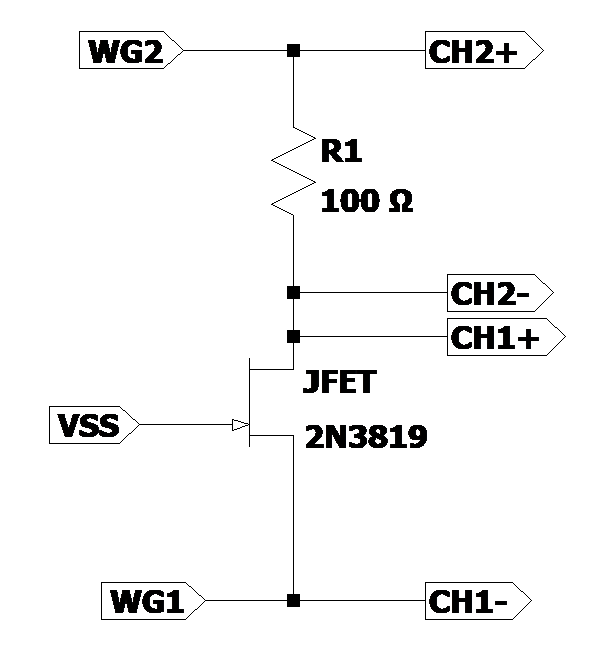
\includegraphics[scale=0.5]{Draft1}
    \caption{Schema circuitale per la verifica di funzionamento del JFET}
\end{figure}
Vista la struttura del jfet, sappiamo che aumentando $V_{GS}$ le zone della giunzione vengono svuotate dai portatori di carica, fino a che non si raggiunge un potenziale di pinch-off $V_p$ in cui il canale risulta completamente svuotato e la corrente di drain tende a 0. Al contrario invece, quando $V_{GS}=0$ il canale risulta "aperto", perciò misureremo in questa situazione il massimo di corrente; quando invece $V_{GS}>V_p$ la corrente sarà pressoché nulla.
Abbiamo quindi inviato a $V_{SS}$ una tensione continua di -5 V, a WG1 una rampa a scalini di 250 mV partendo da -5V fino a 0 V, e a WG2 che per ogni gradino fatto da WG1 genera una rampa che parte dal valore corrente di WG1 e arriva fino a 5V.
Di seguito quello che otteniamo dall'oscilloscopio:
\begin{figure}[H]
    \centering
	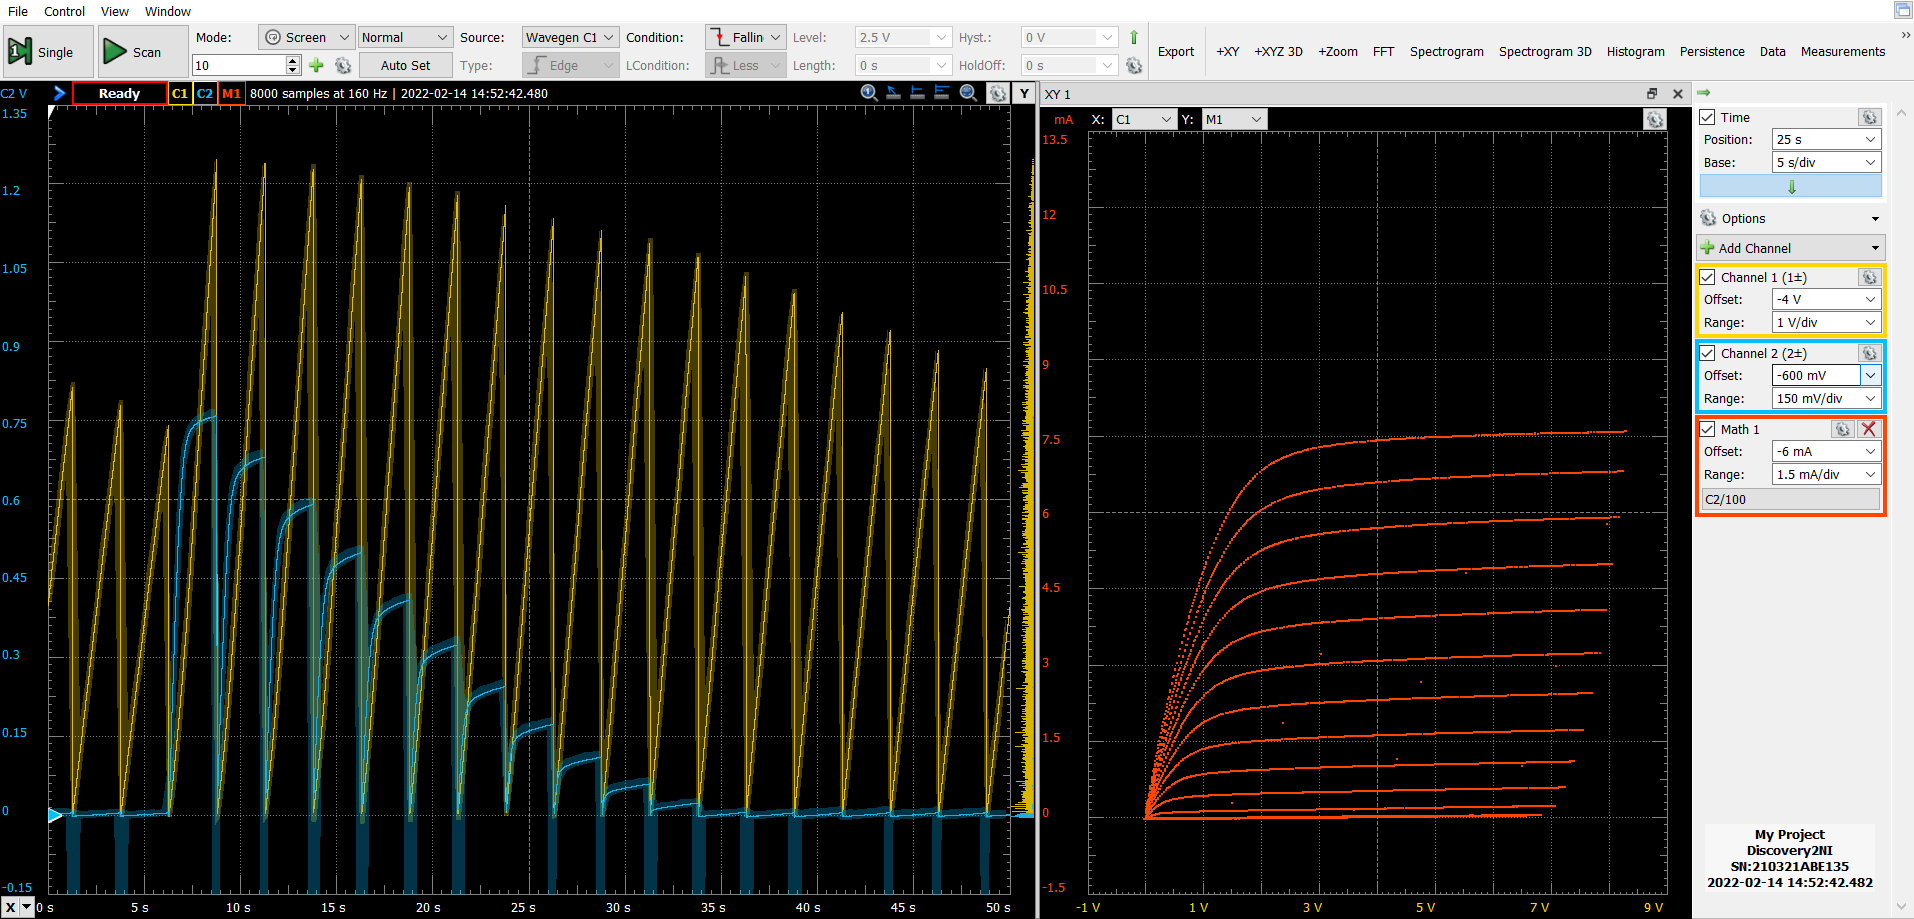
\includegraphics[scale=0.4]{time}
    \caption{Grafici di CH1, CH2 e math1 (definito come CH2/R1) in funzione del tempo}
\end{figure}
\begin{figure}[H]
    \centering
	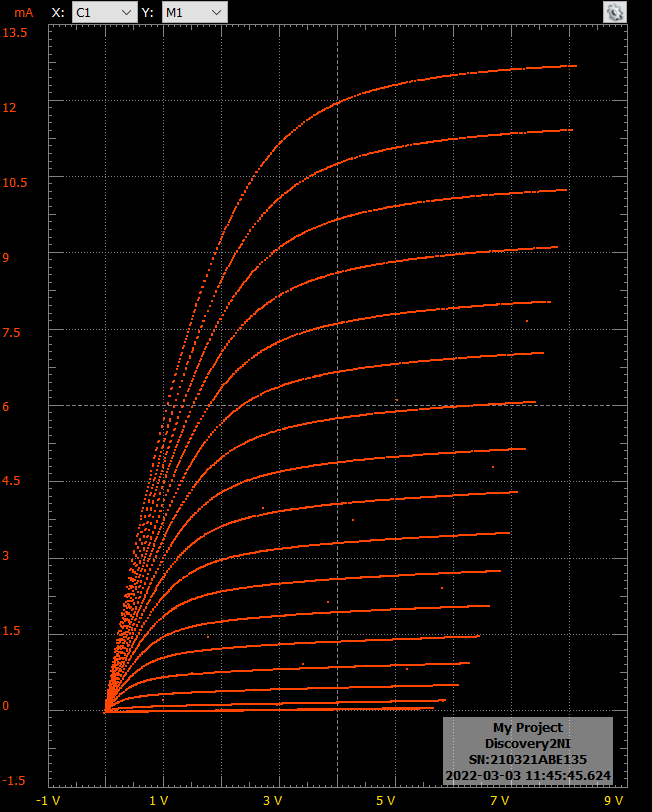
\includegraphics[scale=0.4]{vgs}
    \caption{Curve caratteristiche del jfet per $I_{DS}$ su $V_{DS}$}
\end{figure}
Come detto prima, il momento in cui la corrente è maggiore (nel grafico a sinistra è sufficiente soffermarsi a vedere l'andamento di CH2) si ottiene quando $V_{GS}$ è pari a 0, che nello stesso grafico è quando la rampa di WG2 misurata da CH1 è più alta (perchè in quel caso $V_S$ è pari a $V_G$ ovvero $V_{SS}$.
Inoltre si può vedere che oltre un certo punto l'andamento di CH2 risulta approssimativamente costante: questo si ottiene quando viene superata la tensione di pinch-off, che siamo andati a misurare tramite cursori:
\[
V_p=-4.0 \pm 0.2 V
\]
Infine, sempre utilizzando i cursori, abbiamo misurato la corrente nella traccia in cui $V_{GS}=0$, nel grafico di sinistra è la curva più alta; da cui abbiamo ricavato:
\[
I_{dss}=12.6 \pm 0.2 mA
\]
Confrontando col datasheet risulta che entrambi i valori risultano compatibili con gli intervalli dichiarati dai costruttori (dato che noi abbiamo utilizzato valori di $V_{DS}$ minori di quelli utilizzati nel datasheet)
\section{Amplificatore e punto di lavoro}
A questo punto abbiamo costruito il circuito per l'amplificatore di tensione:
\begin{figure}[htbp]
    \centering
	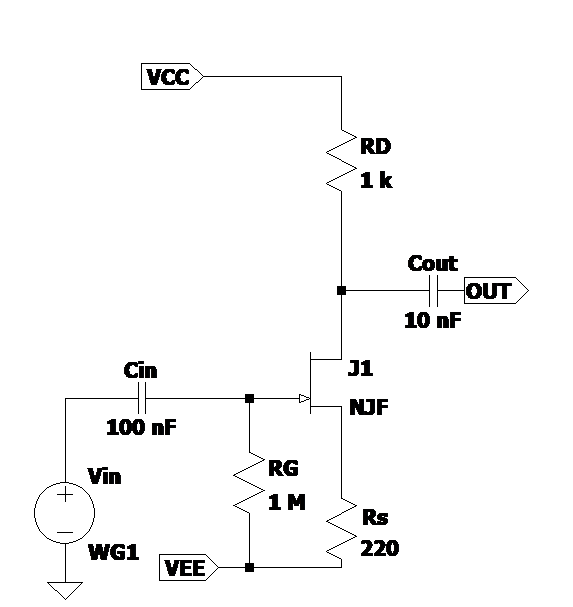
\includegraphics[scale=0.7]{Draft2}
    \caption{Schema circuitale per l'amplificazione di segnale tramite JFET}
\end{figure}
Quindi si è collegato $V_{CC}$ a 5V e $V_{EE}$ a -5V tenendo scollegato $V_{in}$ per verificare il punto di lavoro del JFET.
Misurando la Caduta di potenziale ai capi della resistenza $R_D$ abbiamo calcolato la corrente di quiescenza con la legge di ohm, da cui si ricava $I_{ds}=7.29 \pm 0.07 mA$ che risulta essere circa la metà della $I_{dss}$.
Si è quindi proseguito con la misura di $V_{GS}$ e di $V_DS$ per verificare quello che abbiamo appena misurato.
Sappiamo infatti che dato $V_{GS}$ e $V_p$ e se il JFET è in regime di saturazione:
\begin{equation}
I_{ds}=\frac{I_{dss}}{V_p ^2}(V_{GS}-V_p)^2
\end{equation}
Per misurare $V_{GS}$ abbiamo si è calcolata la differenza tra le misure di $V_G$ e $V_S$:
\[
V_{GS}=-886 \pm 7 mV
\]
\[
V_{DS}=2.35 \pm 0.01 V
\]
Dato che $V_{DS} > V_{GS} - V_p$ si ricava che siamo in zona di saturazione, a questo punto basta applicare l'equazione; si ottiene quindi 
\[
I_{ds}(V_{GS},V_p,I_{dss})=4.14 \pm 0.07 mA
\]
Che risulta essere compatibile con quanto misurato.
Stimiamo infine la transconduttanza tramite la formula
\begin{equation}
g_m = \frac{2 I_{dss}}{|V_p|}\sqrt{\frac{I_{d}}{I_{dss}}}
\end{equation}
da cui ricaviamo $g_m = 4.73 \si{m\mho}$, andando quindi a ricercare nel datasheet il valore fornito da costruttore, troviamo un grafico di $g_m$ in funzione della frequenza a cui opera il JFET, in particolare notiamo che per frequenze minori di circa 500 Mhz la transconduttanza deve essere compresa approssimativamente tra 4 e 5, similarmente anche la transammettenza deve essere compresa tra 3 e 6.5 $\si{m\mho}$; il valore misurato rissulta quindi compatibile.
%=======================
\section{Amplificatore di segnale}
A questo punto si è collegato l'ingresso $V_in$ all'entrata dell'amplificatore, e lo abbiamo pilotato con un'onda sinusoidale di 1 kHz con un'ampiezza compresa tra 100 mV e 2.8 V a passi di 100 mV.
\begin{table}[H]
\centering
\begin{tabular}{cccccc}

$V_{in} [V]$ & $\Delta V_{in}[V]$ & $V_{out} [V]$ & $\Delta V_{out} [V]$ & $|A|$ & $\Delta A$ \\
\midrule
100 m & 1 m  & 206 m & 2 m   & 2.06 & 0.02 \\
200 m & 2 m  & 411 m & 4 m   & 2.05 & 0.02 \\
300 m & 3 m  & 616 m & 7 m  & 2.05 & 0.03 \\
400 m & 4 m  & 821 m & 7 m  & 2.05 & 0.02 \\
501 m & 4 m  & 1.03  & 8 m  & 2.05 & 0.02 \\
601 m & 7 m  & 1.22  & 18 m & 2.04 & 0.04 \\
701 m & 7 m  & 1.42  & 19 m & 2.03 & 0.03 \\
801 m & 7 m  & 1.62  & 20 m & 2.02 & 0.03 \\
901 m & 7 m  & 1.80  & 0.02 & 2.00 & 0.03 \\
1.00  & 8 m  & 1.99  & 0.02 & 1.99 & 0.03 \\
1.10  & 8 m  & 2.16  & 0.02 & 1.96 & 0.02 \\
1.20  & 8 m  & 2.31  & 0.02 & 1.93 & 0.02 \\
1.30  & 9 m  & 2.46  & 0.02 & 1.89 & 0.02 \\
1.40  & 9 m  & 2.59  & 0.03 & 1.86 & 0.02 \\
1.50  & 0.02 & 2.71  & 0.04 & 1.82 & 0.03 \\
1.60  & 0.02 & 2.84  & 0.04 & 1.78 & 0.03 \\
1.70  & 0.02 & 2.93  & 0.04 & 1.72 & 0.03 \\
1.80  & 0.02 & 3.05  & 0.04 & 1.69 & 0.03 \\
1.90  & 0.02 & 3.15  & 0.04 & 1.65 & 0.03 \\
2.00  & 0.02 & 3.25  & 0.04 & 1.62 & 0.03 \\
2.10  & 0.02 & 3.34  & 0.04 & 1.59 & 0.02 \\
2.20  & 0.02 & 3.48  & 0.04 & 1.56 & 0.02 \\
2.30  & 0.02 & 3.53  & 0.04 & 1.53 & 0.02 \\
2.40  & 0.02 & 3.59  & 0.04 & 1.49 & 0.02 \\
2.50  & 0.02 & 3.61  & 0.04 & 1.44 & 0.02 \\
2.60  & 0.03 & 3.63  & 0.04 & 1.39 & 0.02 \\
2.71  & 0.03 & 3.63  & 0.04 & 1.34 & 0.02 \\
2.81  & 0.04 & 3.64  & 0.04 & 1.29 & 0.02 \\
\bottomrule
\end{tabular}
\end{table}
Data la caratteristica del circuito di essere in configurazione common source, possiamo modellare il guadagno come
\begin{equation}
A_v =-\frac{g_m R_d}{1+g_mR_s}
\end{equation}
Utilizzando i dati ottenuti prima possiamo ricavare il valore atteso:
\[
A_v=-2.33 \pm 0.02
\]
Ci accorgiamo subito che questo risultato non risulta essere compatibile con quanto misurato prima.
Essendo il guadagno negativo se ne deduce che l'amplificatore sarà di tipo invertente, cosa che si vede immediatamente dai grafici di $V_{in}$ e $V_{out}$.
\begin{figure}[H]
    \centering
	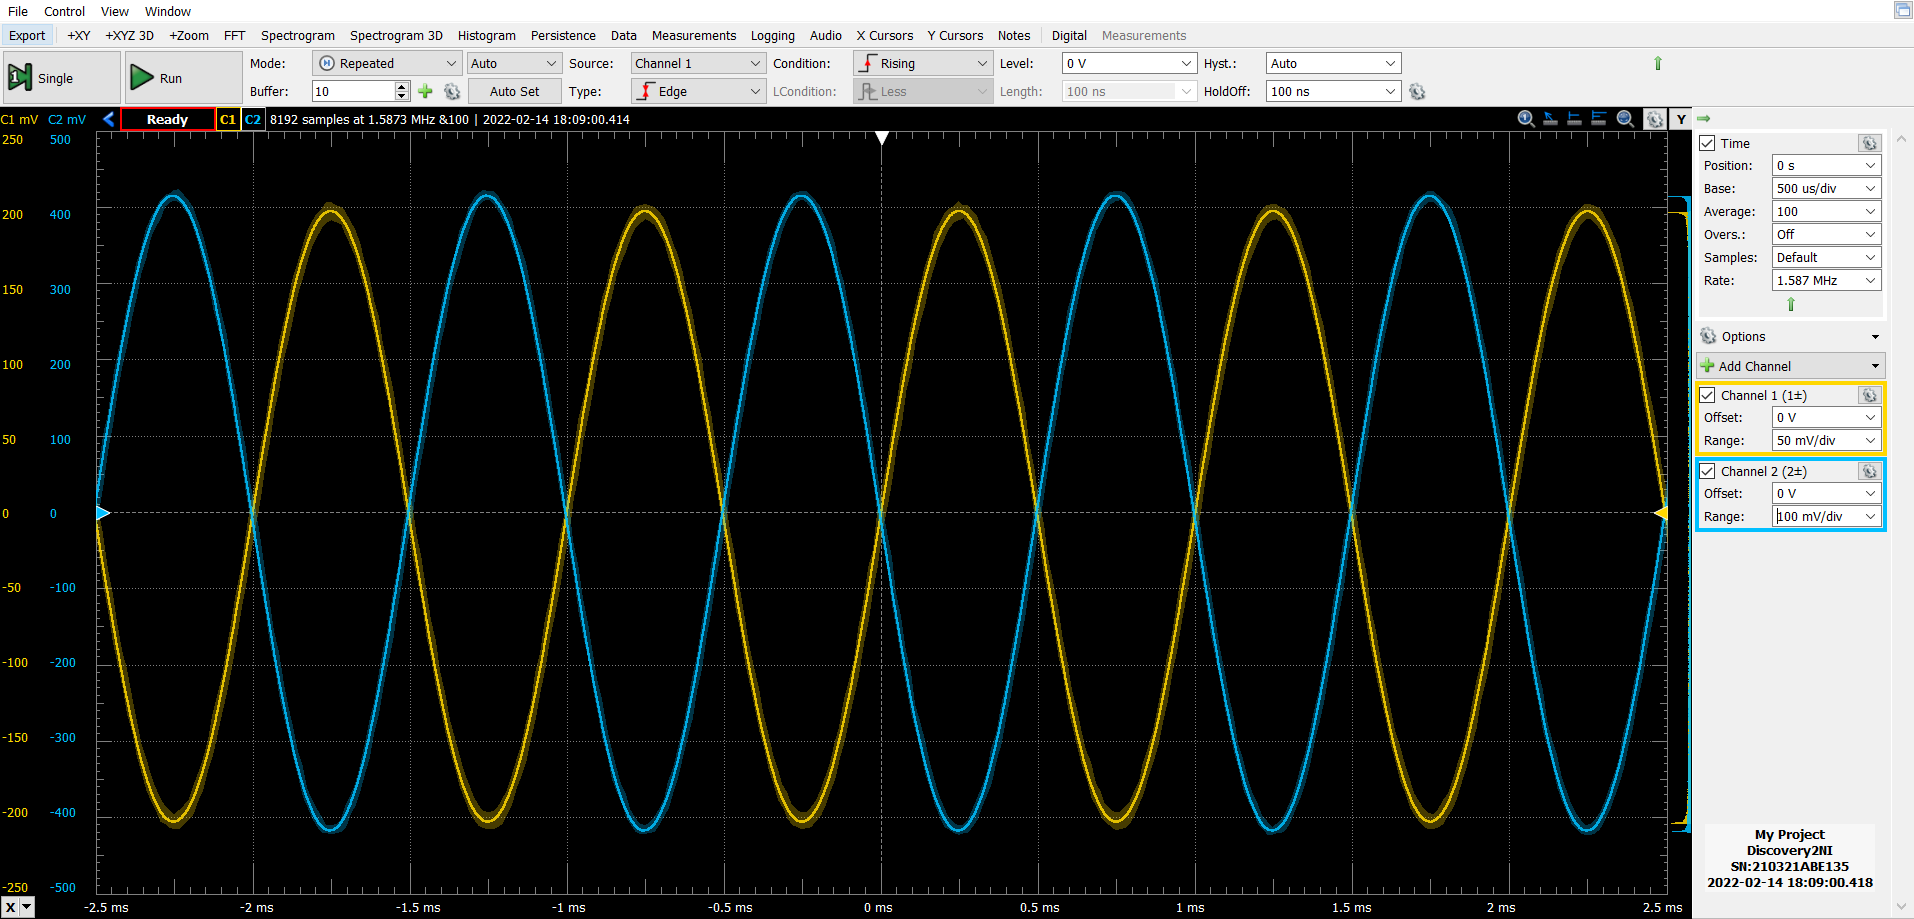
\includegraphics[scale=0.4]{amp.200}
    \caption{Grafici di $V_{in}$ e $V_{out}$ in funzione del tempo con ampiezza $V_{in}=200 mV$}
\end{figure}
\begin{figure}[H]
    \centering
	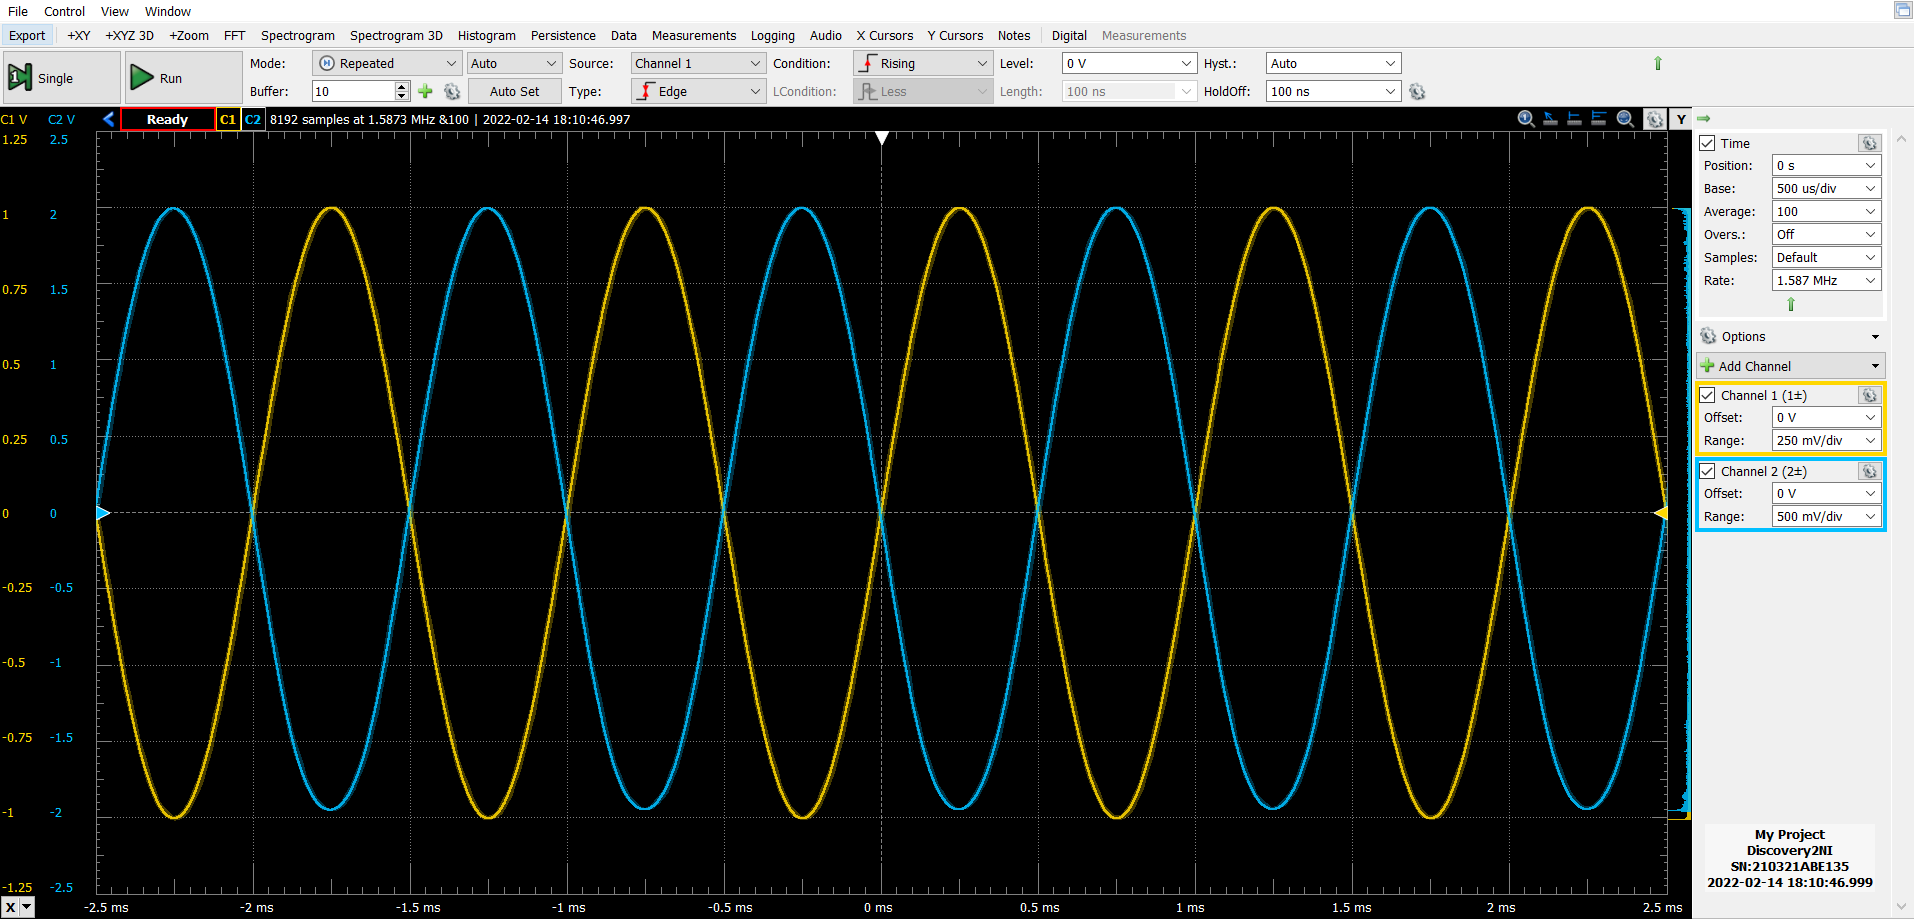
\includegraphics[scale=0.4]{amp.1000}
    \caption{Grafici di $V_{in}$ e $V_{out}$ in funzione del tempo con ampiezza $V_{in}=1000 mV$; in questa situazione si nota una distorsione nel segnale in uscita, in particolare la parte inferiore dell'onda risulta schiacciata verso lo 0}
\end{figure}
\begin{figure}[H]
    \centering
	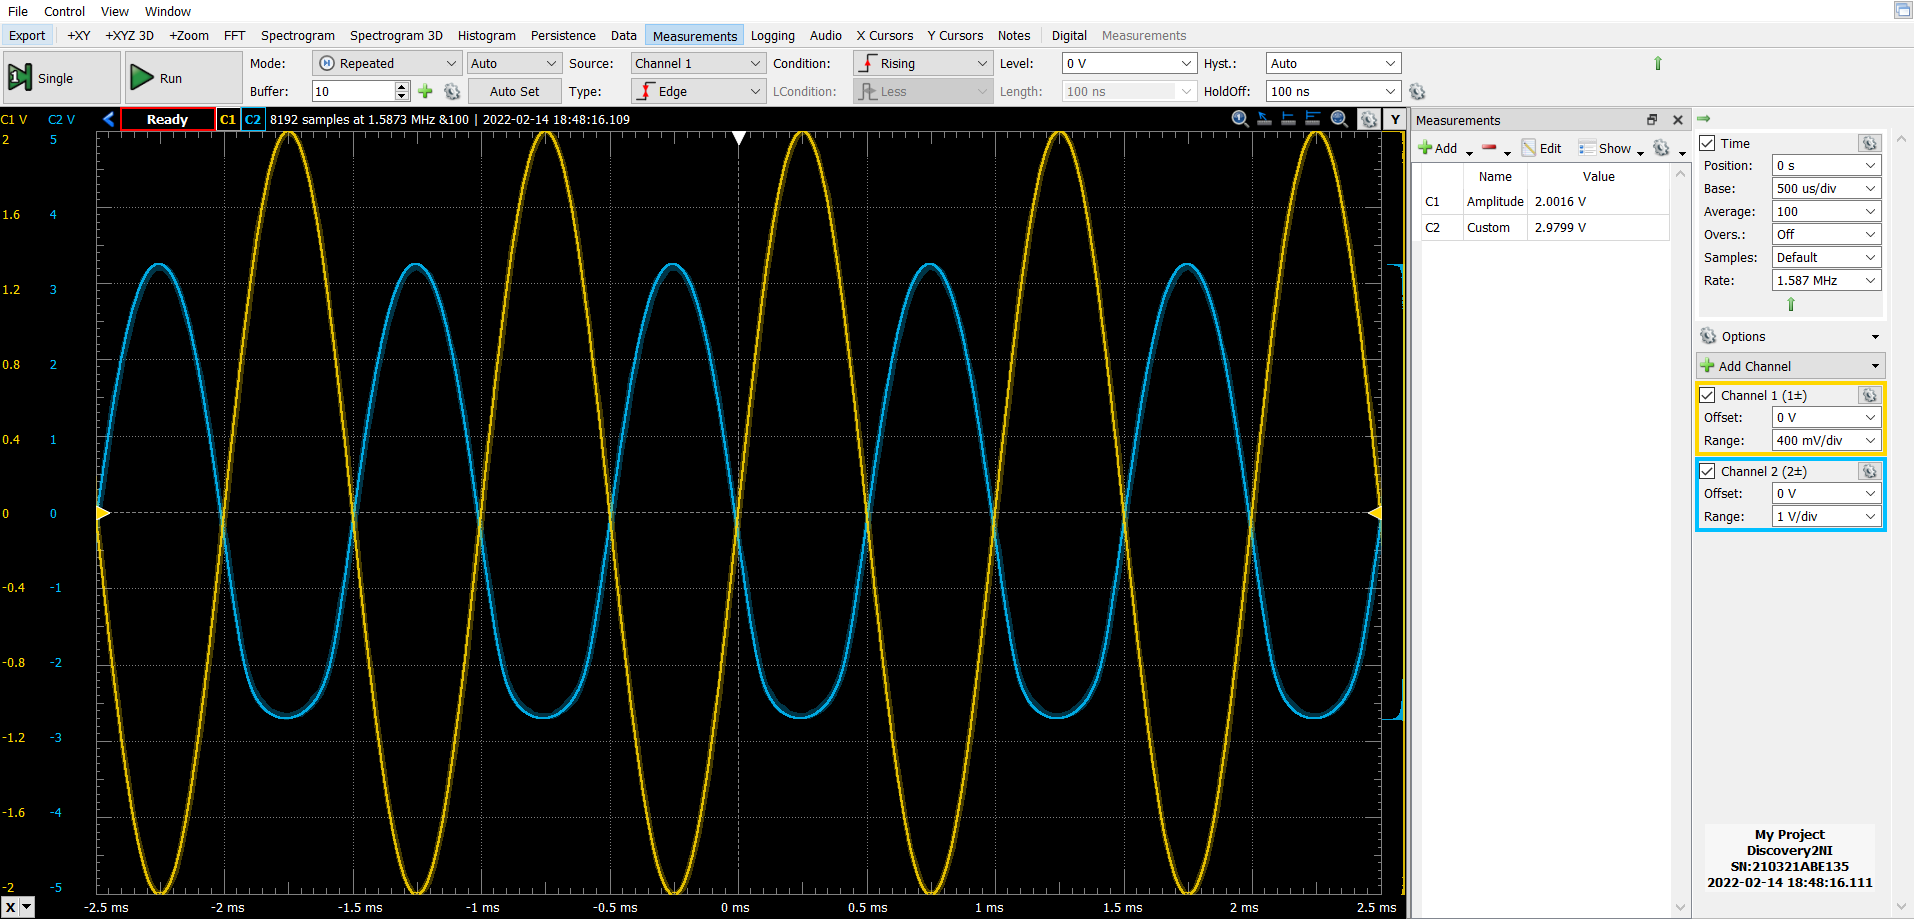
\includegraphics[scale=0.4]{amp.2000}
    \caption{Grafici di $V_{in}$ e $V_{out}$ in funzione del tempo con ampiezza $V_{in}=2000 mV$; qua la distorsione della parte inferiore dell'onda è molto più pronunciata}
\end{figure}
\begin{figure}[H]
    \centering
	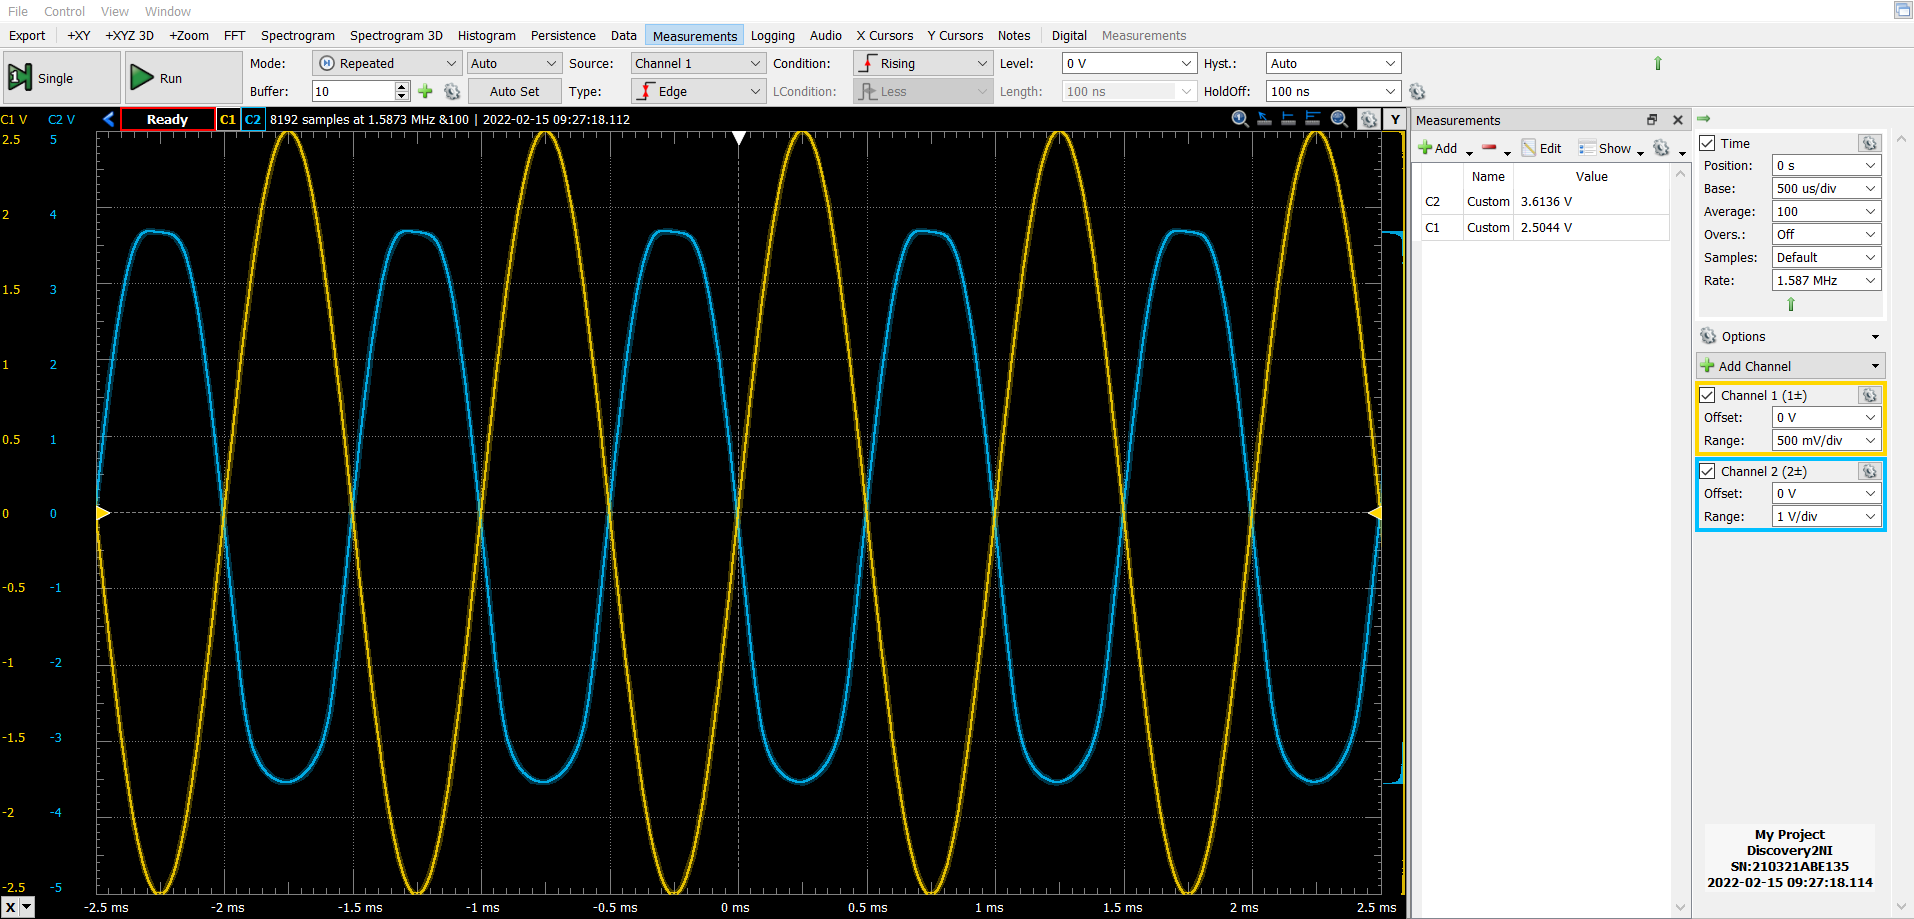
\includegraphics[scale=0.4]{amp.2500}
    \caption{Grafici di $V_{in}$ e $V_{out}$ in funzione del tempo con ampiezza $V_{in}=2500 mV$; si inizia a intravedere un taglio nella parte superiore dell'onda, mentre la parte inferiore risulta ancora distorta}
\end{figure}
\begin{figure}[H]
    \centering
	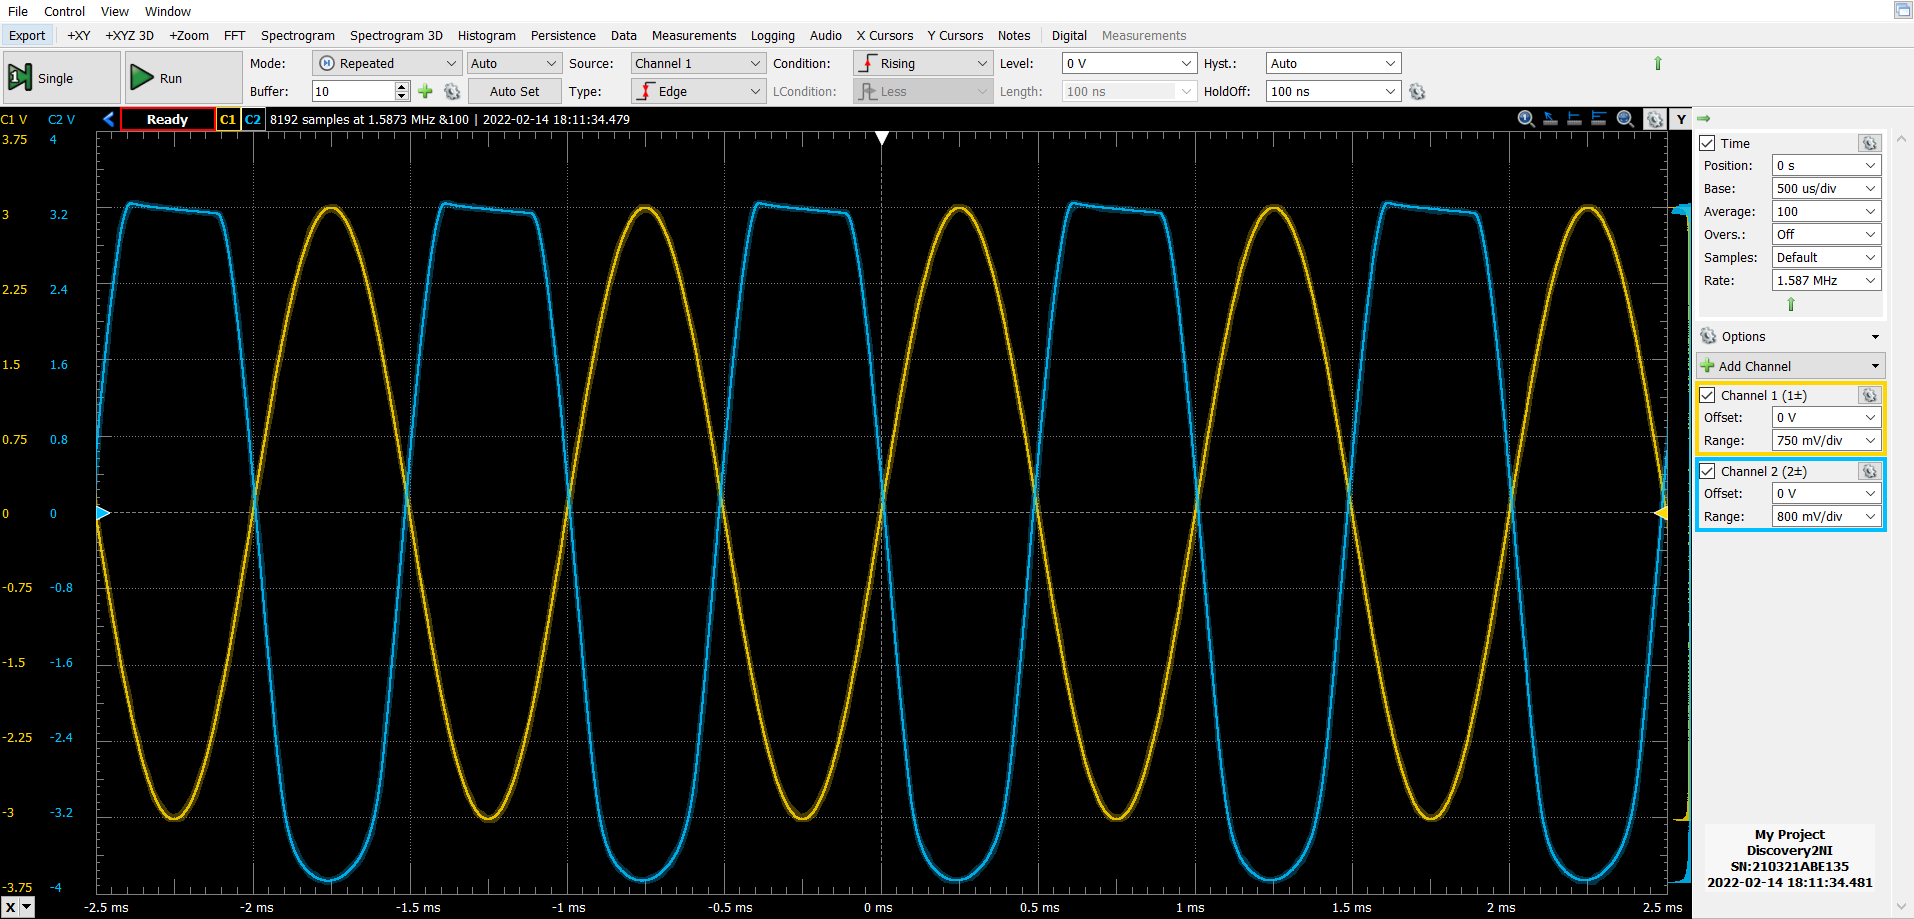
\includegraphics[scale=0.4]{amp.3000}
    \caption{Grafici di $V_{in}$ e $V_{out}$ in funzione del tempo con ampiezza $V_{in}=3000 mV$; il taglio della parte alta dell'onda risulta ora più evidente}
\end{figure}

%=======================
\section{Risposta in frequenza}
Utilizzando lo strumento Network analyzer siamo passati a misurare la risposta in frequenza del circuito tra i 5Hz e i 10 Mhz utilizzando una $V_{in}=200 mV$\\
\begin{figure}[H]
    \centering
	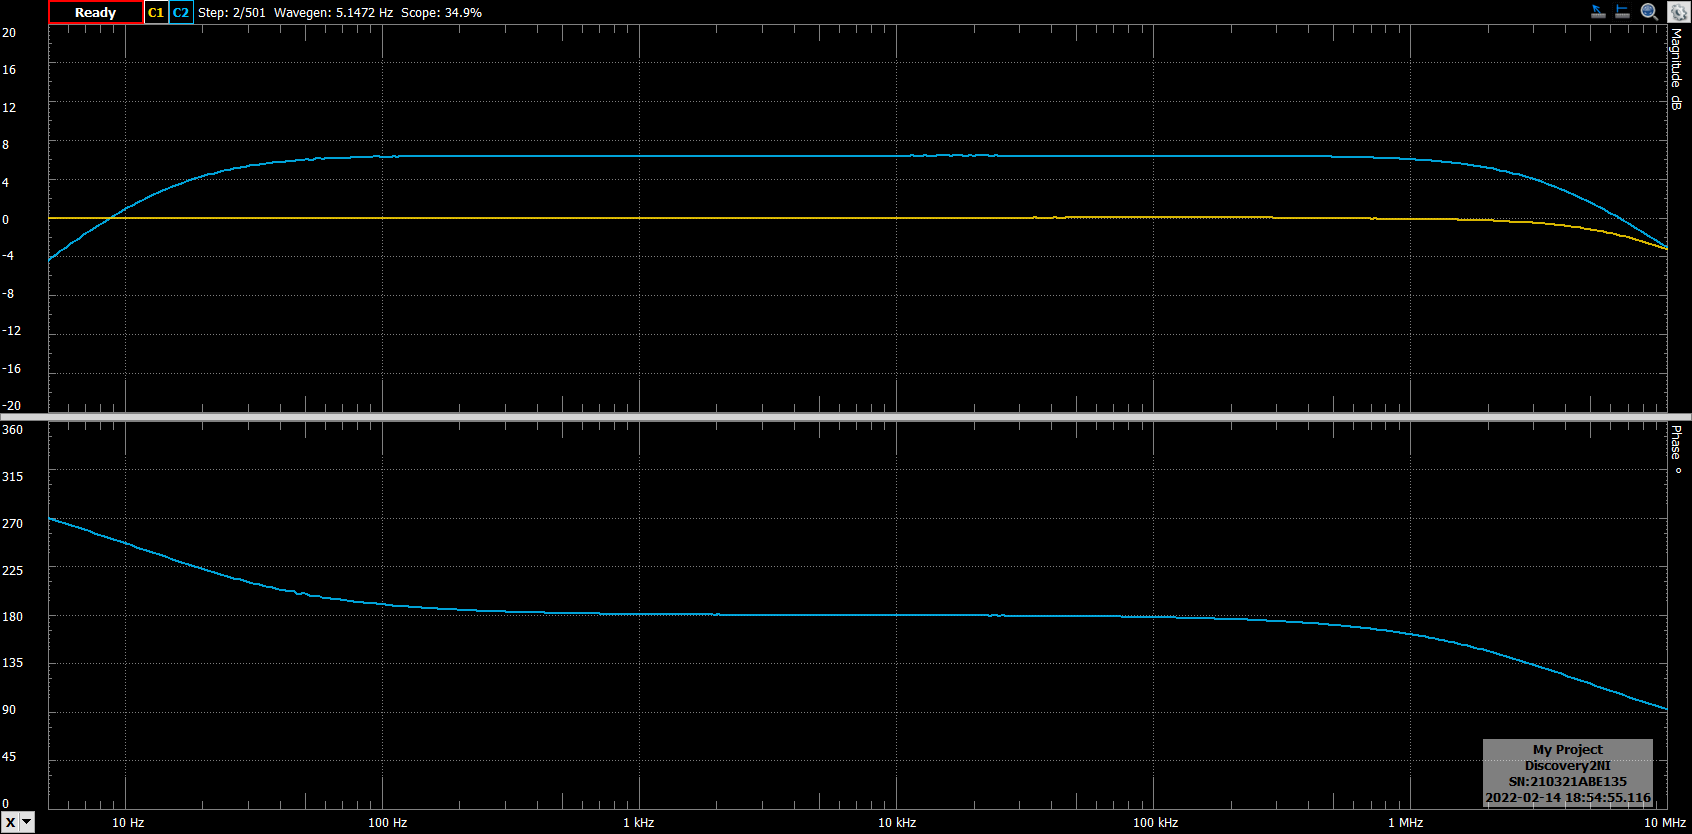
\includegraphics[scale=0.4]{network}
    \caption{Risposta in frequenza del circuito amplificatore a common source}
\end{figure}
Si è quindi misurato il guadagno di centro banda, che risulta essere pari a $6.31 dB$ che convertendolo in $A_v$ si ottiene $2.07$, che risulta compatibile con quanto misurato al punto precedente.
A partire da ciò abbiamo ricavato le frequenze di taglio (basso e alto) tramite cursori, ricercando quando la curva del guadagno vale 3.31 dB:
\[
F_{TA}=3.54 \pm 0.02Mhz
\]
\[
F_{TB}= 16.0 \pm 0.1Hz
\]
%=======================
\section{Aumento del guadagno}
Abbiamo ora inserito un condensatore elettrolitico in parallelo a $R_s$, chiamato $C_E$.
\begin{figure}[H]
    \centering
	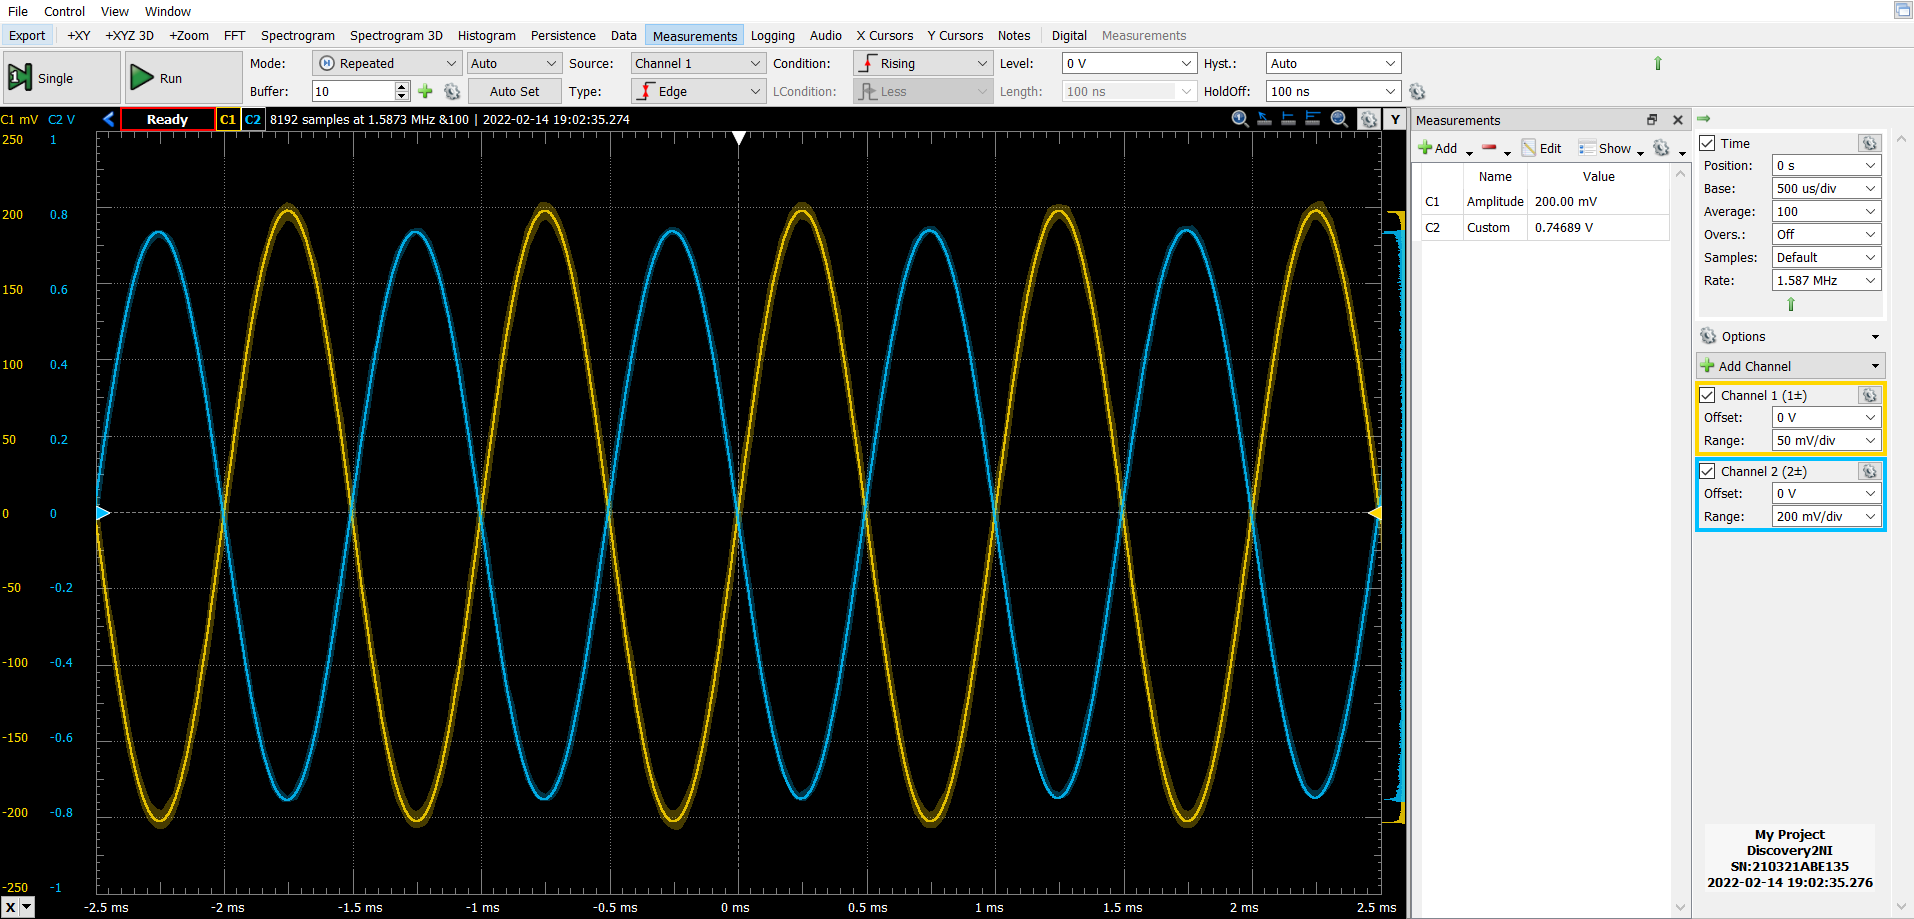
\includegraphics[scale=0.4]{amp.200.cap}
    \caption{Grafici di $V_{in}$ e $V_{out}$ in funzione del tempo con ampiezza $V_{in}=200 mV$ con condensatore elettrolitico $C_E$ in parallelo a $R_s$}
\end{figure}
Aggiungendo il condensatore $C_E$ viene a modificarsi l'impedenza in parallelo con $R_s$, che diminuisce, aumentando così il guadagno
Utilizzando sempre la frequenza di 1 kHz ci si aspetta $A_v =$
Possiamo subito notare che il guadagno è aumentato come ci si aspettava ed è passato ad $A_v =3.20 \pm 0.04$
%=======================
\section{Impedenza in ingresso}
Si è infine provata a misurare l'impedenza in ingresso al circuito mettendo in serie a $V_{in}$ un resistenza $R_S$ dello stesso ordine di grandezza dell'impedenza del circuito attesa, ed utilizzando lo strumento impedance analyzer di waveform in configurazione “W1-C1-R-C2-DUT-GND”; si è così valutata l'impedenza $Z_{IN}$ e la reattanza in parallelo $X_P$ in funzione della frequenza, compresa tra 1 e 10 kHz.
\begin{figure}[H]
    \centering
	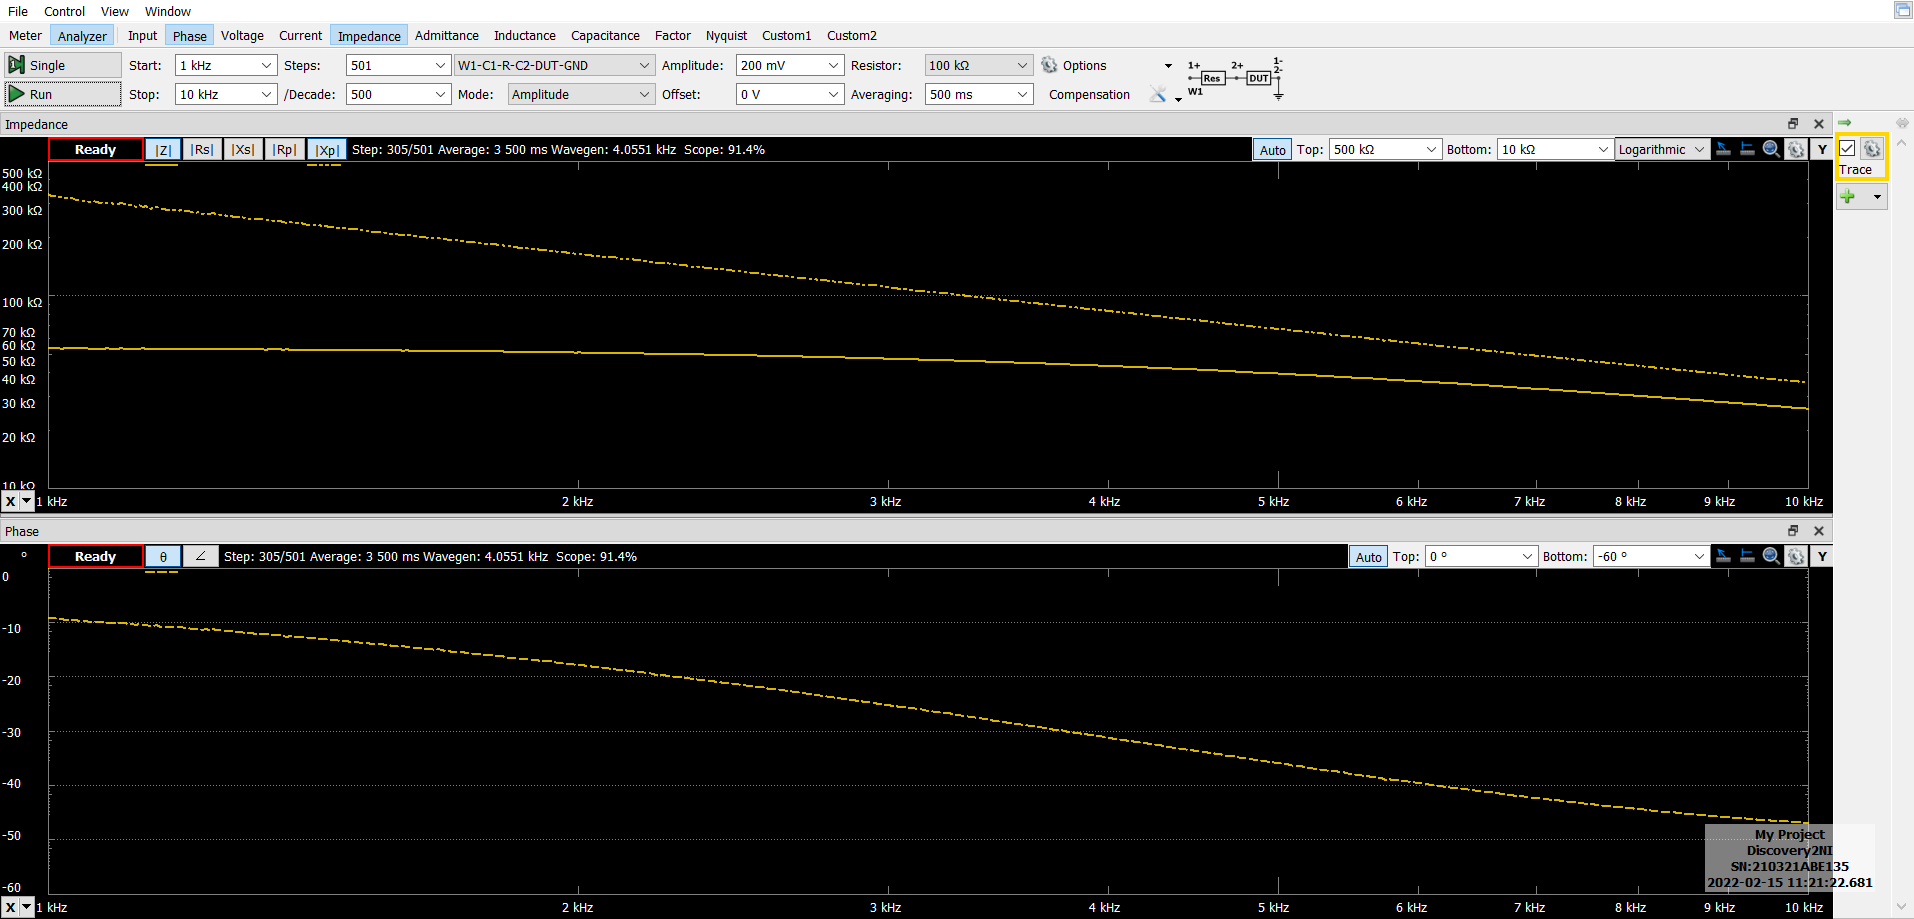
\includegraphics[scale=0.4]{impedance}
    \caption{Grafici di impedenza in ingresso e reattanza parallelo in funzione della frequenza per $R_S=100 \si{k\ohm}$}
\end{figure}
%=======================
\section*{Conclusioni e commenti finali}


%=======================
\section*{Dichiarazione}
I firmatari di questa relazione dichiarano che il contenuto della relazione \`e
originale, con misure effettuate dai membri del gruppo, e che tutti i firmatari
hanno contribuito alla elaborazione della relazione stessa.


\end{document}
